\documentclass{article}
\usepackage[a4paper, total={6in, 8in}]{geometry}
\usepackage[utf8]{inputenc}
\usepackage[T1]{fontenc}
\usepackage[english]{babel} % If you write in English
\usepackage{a4wide}

\usepackage{graphicx} %per les fotos
\usepackage[pdftex]{hyperref}
\usepackage{color}
\hypersetup{%
colorlinks=true,
linkcolor=black,
citecolor=black,
urlcolor=blue}
\usepackage{enumitem}
\setlist[description]{leftmargin=\parindent,labelindent=\parindent}
\setlist{itemsep=1pt,parsep=1pt}

\title{Information criteria and convergence assessment tools for
ArviZ}
\author{Oriol Abril}
\date{April 2019}

\begin{document}

\maketitle

\section{Abstract}\label{abstract}

ArviZ is a Python package for exploratory analysis of Bayesian models,
from diagnostics to visualization. It is designed as a backend-agnostic
tool with the goal to reach the widest user base and thus contribute to
extend best practices among Bayesian inference practitioners.

Two key problems in this field are model comparison and convergence
analysis. Model comparison is not trivial because of the different
structures and number of parameters of each model. Fortunately, there
are some information criteria (i.e.~leave-one-out (LOO)
cross-validation) that can be used for this task. Even though
convergence is proven for infinite iterations, it is not the case for
finite MCMC runs, which can be arbitrarily bad. Convergence assessment
must take into account both intra- and inter-chain correlations.

ArviZ implements many of these algorithms for diagnostic and comparison,
at least at a preliminary level, but it still lacks plots and tools to
ease and improve its interpretation. This project seeks to design and
implement these tools. Moreover, it will pay special attention to
testing and documentation with examples not only of the new
functionalities, but also of the already implemented ones.

\section{Technical Details}\label{technical-details}

This project will analyze the diagnostic and statistical functions in
ArviZ to assess the stage they are in. In addition, there are some plots
related to the interpretation of these functions (i.e.
\texttt{plot\_khat} or \texttt{plot\_autocorr}) which will also be
analyzed (and created if any relevant function is missing, which for
example, may be the case of the LOO probability integral transformation
(PIT) plot requested in
\href{https://github.com/arviz-devs/arviz/issues/80}{\#80}). Each of
these functions should (in decreasing priority):

\begin{enumerate}
\def\labelenumi{\arabic{enumi}.}

\item
  Be implemented coherently within ArviZ API. More specifically, for
  statistical functions, take as input an InferenceData object or xarray
  and return structured and easily interpreted data.
\item
  Have a docstring detailing its use, inputs and outputs
\item
  Have tests covering the most frequent use cases. This includes
  checking different parameter combination and warning messages, if
  appliable
\item
  Include examples on its usage, notes on its implementation (if
  appliable) and references in docstring
\item
  Be thoroughly explained in
  \href{https://github.com/arviz-devs/arviz_resources}{arviz\_resources}
\end{enumerate}

Therefore, this project will require intensive usage of many external
libraries, such as \texttt{xarray}, \texttt{sphinx}, \texttt{pytest} and
in less extent \texttt{matplotlib}. GitHub issues will also play a key
role in discussing ArviZ's API (i.e.
\href{https://github.com/arviz-devs/arviz/issues/501}{\#501}, or
\href{https://github.com/arviz-devs/arviz/issues/415}{\#415}). It will
also be essential to have a deep understanding of the mathematics behind
the algorithms in order to write relevant examples and documentation.

\section{Schedule of Deliverables}\label{schedule-of-deliverables}

The project will start with a design phase to decide with the core
developers and the community which functions (if any) should be added to
ArviZ and to agree on a unique API. In addition, while working on these
two deliverables, I will familiarize myself with the algorithms and
libraries used in the project.

The second phase will build on top of the previous deliverables,
guaranteeing that all selected functions fulfill points 1-3 (as
explained above). I will start with information criteria (IC) related
functions and afterwards work with MCMC diagnostics.

Eventually, point 4 will be tackled for as many functions as possible.
However, point 5 will be adressed following the draft of its table of
contents one subject at a time in order to ensure the quality and
thoroughness of the resources written.

\begin{figure}[!htb]
\centering
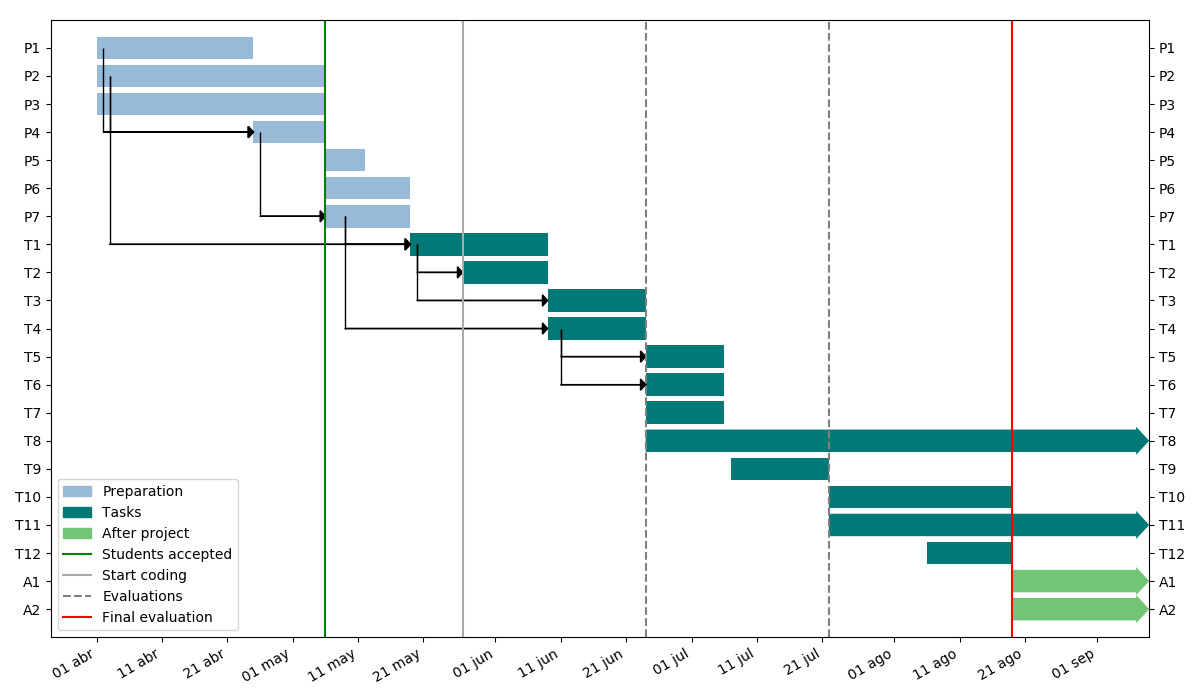
\includegraphics[width=\linewidth]{gantt.png}
\caption{Planned project schedule. The color code indicates preparation for the coding period, coding period tasks and contributions after the project ends. In addition, the vertical lines show the key dates of the program.}\label{gantt}
\end{figure}

\subsection{\texorpdfstring{\textbf{Community Bonding Period} (before
May
19th)}{Community Bonding Period (before May 19th)}}\label{community-bonding-period-before-may-19th}

\begin{description}
\item[P1] Familiarize with the needed libraries: ArviZ, pytest, xarray,
  sphinx
\item[P2] Familiarize and understand all the algorithms involved
  \begin{itemize}
    \item Read references in ArviZ docs and in issues requesting new stats or
  diagnostic features
    \item Read ArviZ's or similar libraries implementation
  \end{itemize}
\item[P3] Contribute to ArviZ tests, preferably but not exclusively to
  project related functionalities.
\item[P4] Create a proposal for functions to add to ArviZ and for the unique
  API
\item[P5] Decide the methodology to include the work in the
  \href{https://google.github.io/gsocguides/student/evaluations\#final-evaluations-and-work-product-submission}{final
  evaluation}
\item[P6] Write examples of existing IC functions
\item[P7] Participate in the discussion of API and functions design and
  decide on one of the alternatives
\end{description}\vspace{1ex}


\noindent Expected results:

\begin{itemize}
\item
  Reading literature and implementation of the algorithms that will be
  used is essential to understand them and to asses which ones should be
  present in ArviZ.
\item
  Reading ArviZ implementation of the already present functions will
  also be a way to check their documentation.
\item
  Working with tests will provide me with hands on experience with the
  code, with the extra advantage of making error detection easier in the
  next steps of the project.
\item
  One (or several) issue with the proposal for the functions to add to
  ArviZ and for the API (i.e. \texttt{plot\_khat} and
  \texttt{plot\_autocorr} both need to execute a stats/diagnostics
  function before plotting, \texttt{plot\_khat} makes the used execute
  the function and its input is not InfereceData whereas
  \texttt{plot\_autocorr}'s input is InferenceData and calls the
  autocorr function itself).
\end{itemize}

\subsection{\texorpdfstring{\textbf{Phase 1} (May 20th - August
19th)}{Phase 1 (May 20th - August 19th)}}\label{phase-1-may-20th---august-19th}

\begin{description}
\item[T1] Implement and document IC functions
\item[T2] Write their tests
\item[T3] Write IC examples
\item[T4] Guarantee documentation and tests of MCMC diagnostics (and
  implementation if appliable)
\item[T5] Guarantee tests for MCMC diagnostics
\item[T6] Guarantee examples for MCMC diagnostics
\item[T7] Check behaviour in a wide range of real cases (extra examples and
  possible issues from ArviZ prereleases users)
\item[T8] Correct bugs
\item[T9] Profile memory and cpu usage to identify possible bottlenecks
\item[T10] Write a draft of one related section in ArviZ-resources
  (optional)
\item[T11] Finish or continue working on any pending task
\item[T12] Write Google Summer of Code final evaluation
\end{description}

\subsection{\texorpdfstring{\textbf{After
GSoC}}{After Google Summer of Code}}\label{after-gsoc}

\begin{description}
\item[A1] Finish the still pending goals if any.
\item[A2] Contribute solving bugs on the created functions and answering
  issues about their usage.
\end{description}

\section{Why me?}\label{why-me}

My name is Oriol Abril. I graduated from Engineering Physics at
Polytechnical University of Catalonia in 2017. I am currently graduating
in High Enegry Physics, Astrophysics and Cosmology at the Autonomous
University of Barcelona. Since my first research experience in 2013, I
have made use of multiple programming languages, including Python,
Matlab or Fortran. Many of my projects have involved Bayesian inference,
especially with \href{https://emcee.readthedocs.io/en/latest/}{emcee}.
Upon discovering ArviZ nearly a year ago and realizing its power with
regard to my inference results -in storing, plotting, or comparing them,
among other aspects- I began to extensively use it.

\subsection{Development Experience}\label{development-experience}

I have worked in many projects related with scientific programming, not
only during my undergraduate and graduate studies, but also in
extracurricular activities such as collaborations with the
\href{https://www.isis.stfc.ac.uk/Pages/Molecular-Spectroscopy.aspx}{Molecular
Spectroscopy Group} at the ISIS neutron source and with the High Energy
Physics Institute (\href{http://www.ifae.es/eng/}{IFAE}). In addition, I
have participated actively in
\href{https://stackoverflow.com/users/2504700/xg-plt-py}{StackOverflow},
mainly in questions related to matplotlib, numpy, pandas and
vectorization. I have used ArviZ for my Master's Thesis and, as a
result, I am familiar with most of its functions and API.

\noindent Moreover, I have already contributed to ArviZ:

\begin{itemize}
\item Documentation
  \begin{description}
    \item[\href{https://github.com/arviz-devs/arviz/pull/436}{\#436}] Add emcee
    and pyro cookbook examples {[}MERGED{]}
    \item[\href{https://github.com/arviz-devs/arviz/pull/616}{\#616}] Update
    Docker instructions {[}MERGED{]}
    \item[\href{https://github.com/arviz-devs/arviz/pull/630}{\#630}] 3
      documentation issue fixes {[}OPEN{]}
    \item[\href{https://github.com/arviz-devs/arviz/pull/638}{\#638}] Add
        \texttt{from\_emcee} inline examples {[}OPEN{]}
  \end{description}
\item Testing
  \begin{description}
    \item[\href{https://github.com/arviz-devs/arviz/pull/624}{\#624}] Helper
    method for tests {[}MERGED{]}
  \end{description}
\item IO
\begin{description}
  \item[\href{https://github.com/arviz-devs/arviz/pull/426}{\#426}] emcee
  version 3 compatibility {[}MERGED{]}
  \item[\href{https://github.com/arviz-devs/arviz/pull/450}{\#450}] Update
    \texttt{io\_pyro} to pyro 0.3 release {[}MERGED{]}
  \item[\href{https://github.com/arviz-devs/arviz/pull/550}{\#550}] Emcee
      reader support {[}MERGED{]}
\end{description}
\item Plotting bugs:
\begin{description}
  \item[\href{https://github.com/arviz-devs/arviz/pull/615}{\#615}] \texttt{plot\_pair} return value {[}MERGED{]}
  \item[\href{https://github.com/arviz-devs/arviz/pull/619}{\#619}] Remove
    \texttt{plot\_density} tight\_layout {[}MERGED{]}
  \item[\href{https://github.com/arviz-devs/arviz/pull/637}{\#637}] Fix
    \texttt{plot\_pair} issue and add extra options to \texttt{plot\_kde}
    {[}OPEN{]}
\end{description}
\item Other
\begin{description}
  \item[\href{https://github.com/arviz-devs/arviz/pull/620}{\#620}] Add
  logging arviz wide {[}OPEN{]}
\end{description}
\end{itemize}

\subsection{Other Experiences}\label{other-experiences}

In addition to my academic background and programming experience, I have
also performed extensive courses in Probability, Statistics, Algebra,
Numerical Computation and related subjects during my undergraduate and
graduate studies.

\section{Why ArviZ?}\label{why-arviz}

I have always been really interested in modelling and inference,
specifically in Bayesian modelling. In my research projects, I have come
to realize that in many cases modelling is treated as a limited set of
models and techniques \emph{universally} appliable, either disregarding
or not even knowing the limitations of the models and algorithms used. I
believe that ArviZ is capable of extending and explaining Bayesian
modelling techiques to a really wide community. It will approach many
algorithms and best practices to people with limited programming
habilities, together with a thorough documentation, which will cover its
uses and limitations.

\end{document}
